\chapter{Case Study}
When talking about animal movement behavioural animals might use a reaction-diffusion process. This process entails the movement (diffusion) and the interaction with the environment (reaction). Reaction is often described as finding food, mating a mate or finding a predator. All of these things force the animal into changing its movement behaviour. This could mean a stop in a long search for example. Reaction behaviour will not be a part of this report.

\section{Diffusion processes}
Diffusion processes can also be called walks. This section seeks to explain some of the different walks and what is characteristic about them.

\subsection{Brownian motion}
Brownian motion is a type of random walk where the motion follows a Gaussian distribution. In mathematically terms this can be shown as follows:
\begin{equation}
$Pathlength $ \sim \mathcal{N}(0,t-s) ($for $ 0 \leq s \leq t)
\label{eq:brownianm}
\end{equation}
This type of diffusion where the variance grows over time is called normal diffusion. Characteristic for the Brownian motion is that the walker will return to the same spot multiple times. This can be seen in a 1D model in figure \ref{fig:brownianrw}.
\begin{figure}[H]
\centering
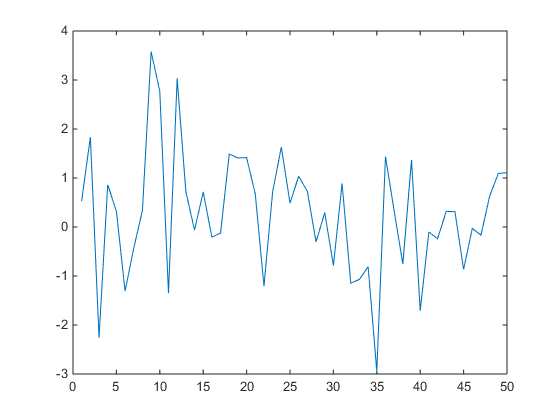
\includegraphics[width = 0.6\textwidth]{billeder/brownian}
\caption{Brownian Random Walk}
\label{fig:brownianrw}
\end{figure}
When looking at Brownian random walks it becomes apparent that the model might not reflect animal behaviour as it would be a bad strategy to visit the same area multiple times in a search. Only when you revisit a site with fast food regeneration would this strategy seem feasible.\\
Brownian motion obeys the rule of the central limit theorem. When the variance in equation \ref{eq:brownianm} gets sufficiently large the distribution will be very wide and the probability for $P(0)$ will be very low.

\subsection{Levy motion}